\documentclass[a4paper, 10pt]{report}
\usepackage{common}
\usetikzlibrary{petri,positioning}

% Cuerpo
\begin{document}

% Carátula
\title{
    III\\
    Programación Concurrente\\
    \large Clases 7 a 9: Memoria distribuida
}
\author{Ramiro Martínez D'Elía}
\date{2021}
\maketitle

% Índice
\tableofcontents

\chapter{Programa distribuido}

\section{Definición}

Los mecanismos de sincronización vistos hasta ahora, están pensados para programas concurrentes que ejecutan en hardware con procesadores que comparten memoria (arquitecturas de memoria compartida).

Sin embargo, hay arquitecturas donde los CPU solo comparten una red de comunicación. Bajo este contexto, los procesos ya no comparten variables sino que comparten \textbf{\emph{canales}}.

Los \textbf{\emph{canales}} son abstracciones de una red de comunicación física y al ser el único recurso compartido entre procesos, toda variable es local a un solo proceso y solo accedida por ese proceso. Esto descarta la necesidad de exclusión mutua.

La ausencia de variables compartidas, permite que los procesos puedan ejecutarse en procesadores distribuidos. Por esta razón, los programas concurrentes que utilizan pasaje de mensajes son llamados \textbf{\emph{programas distribuidos}}.

\section{Canales}

Los canales son \textbf{\emph{estructuras FIFO}} (First In First Out) que contienen mensajes pendientes. Estas estructuras soportan 2 (dos) \textbf{operaciones atómicas \emph{send} y \emph{receive}}. Para iniciar una comunicación, un proceso envía un mensaje por el canal; y otro lo adquiere recibiendolo desde el mismo canal.

La operación \textbf{\emph{send}} puede ser \textbf{asincrónica} (no demora al proceso que la invoca) y \textbf{sincrónica} (demora al proceso que la invoca, hasta que su mensaje fuese recibido). La operación \textbf{\emph{receive}} \textbf{siempre demora} al proceso que la invoca.

La estructura FIFO y la atomicidad de las primitivas send y receive aseguran que; los mensajes eventualmente serán recibidos, los mensajes no serán corrompidos y serán entregados en el orden en que fueron encolados.


\begin{lstlisting}[multicols=2]
channel ch1(string),
        ch2(string);

Program Uno
    string respuesta;
    send ch2("Hola");
    receive ch1(respuesta);
End.

Program Dos
    string saludo;
    receive ch2(saludo);
    send ch1("Aca esta tu respuesta ...);
End.
\end{lstlisting}

Según la forma en que se utilicen, los canales, pueden clasificarse en los siguientes tipos:

\begin{itemize}
    \item \textbf{Mailbox}: Cualquier proceso puede enviar y recibir datos, por alguno de los canales declarados. Relación \emph{n:n}.
    \item \textbf{Input Port}: El canal tiene un único receptor y \emph(n) emisores. Relación \emph{1:n}.
    \item \textbf{Link}: El canal tiene un único receptor y un único emisor. Relación \emph{1:1}.
\end{itemize}

\chapter{Patrones de resolución}

Los tipos de procesos que podemos encontrar en los programas distribuidos, son los mismos que en un programa concurrente con memoria compartida (peers, filters, clientes y servidores).
Lo mismo ocurre, con los patrones de resolución.

A continuación, abordaremos un patrón en particular: \textbf{\emph{interacting peers}}, donde se describirá la forma de interconexión entre procesos. Todos los ejemplos, implementan \textbf{\emph{pasaje de mensajes asincrónicos (PMA)}}.

\begin{basic_box}
    \faIcon[regular]{gem} Soluciones para ordenar números: Merged Network, Odd/Even Exchange Sort, Pipeline. ¿Cantidad de procesos? ¿Cantidad de mensajes? (Ver apunte de gemas).
\end{basic_box}

\section{Iteracting peers: intercambiando valores}

Supongamos el problema donde existen \textbf{\emph{n}} procesos, cada uno con un valor local \textbf{\emph{v}}. El objetivo es, lograr que todos los procesos conozcan el máximo y mínimo valor de \textbf{\emph{v}} de entre todos.

En este caso, los procesos son identicos. Por lo cual, podemos diseñar una solución basada en el esquema de pares que interactúan. 

A contuniación se detallan soluciones, empleando 3 (tres) formas distintas de conexión entre procesos: \textbf{\emph{centralizada}}, \textbf{\emph{simétrica}} y \textbf{\emph{circular}}.

\subsection{Solución centralizada}

En esta solución, utilizaremos un proceso central que; recibirá los valores de los demás. Computará los máximos y mínimos e informará al resto.

\begin{multicols}{2}
\begin{lstlisting}
channel values(int),
        results[n](int, int);
    
Process Peer[i = 1 to n-1]
    int v, min, max;
    send values(v);
    receive results[i](min, max);
End.

Process CentralPeer[0]
    int v, min, max, temp;

    for(i=1 to n-1)
        receive values(temp);
        # Compara y actualiza ...
    end;

    for(i=1 to n-1)
        send results[i](min, max);
End.
\end{lstlisting}

\columnbreak

\centering
\vspace*{\fill}
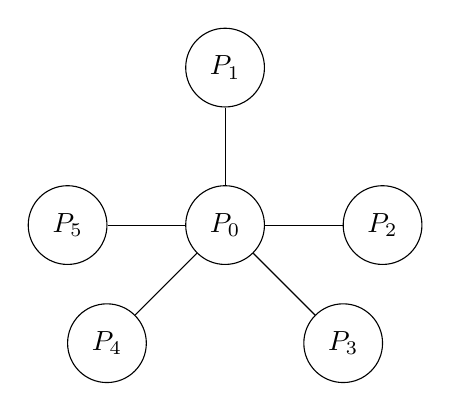
\begin{tikzpicture}
    \node[circle,draw, minimum size=1cm] (0) at (0,0) {$P_0$};
    \node[circle,draw, minimum size=1cm] (1) at (0,2) {$P_1$};
    \node[circle,draw, minimum size=1cm] (2) at (2,0) {$P_2$};
    \node[circle,draw, minimum size=1cm] (3) at (1.5, -1.5) {$P_3$};
    \node[circle,draw, minimum size=1cm] (4) at (-1.5,-1.5) {$P_4$};
    \node[circle,draw, minimum size=1cm] (5) at (-2, 0) {$P_5$};
    \draw (0) -- (1);
    \draw (0) -- (2);
    \draw (0) -- (3);
    \draw (0) -- (4);
    \draw (0) -- (5);
\end{tikzpicture}
\vspace*{\fill}
\end{multicols}

\subsection{Solución simétrica}

En esta solución, todos los procesos realizan el mismo algoritmo. Cada par de procesos, se encuentran conectados mediante un canal.

Cada proceso, envía los datos al resto, y así cada uno puede conocer todos los valores y efecturar el cálculo de máximos y mínimos en paralelo.

\begin{multicols}{2}
\begin{lstlisting}
channel values[n](int, int);

Process Peer[i = 0 to n]
    int v, min, max, temp;

    for(j=0 to n st j != i)
        send values[j](v);

    for(j=0 to n st j != i)
        receive receive[i](temp)
        # Compara y actualiza.
End.
\end{lstlisting}

\columnbreak
    
\centering
\vspace*{\fill}
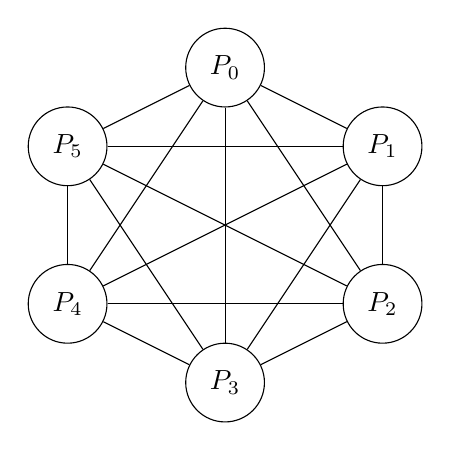
\begin{tikzpicture}
    \node[circle,draw, minimum size=1cm] (0) at (0,2) {$P_0$};
    \node[circle,draw, minimum size=1cm] (1) at (2,1) {$P_1$};
    \node[circle,draw, minimum size=1cm] (2) at (2,-1) {$P_2$};
    \node[circle,draw, minimum size=1cm] (3) at (0, -2) {$P_3$};
    \node[circle,draw, minimum size=1cm] (4) at (-2,-1) {$P_4$};
    \node[circle,draw, minimum size=1cm] (5) at (-2, 1) {$P_5$};
    \draw (0) -- (1); \draw (0) -- (2); \draw (0) -- (3); \draw (0) -- (4);
    \draw (0) -- (5); \draw (1) -- (2); \draw (1) -- (3); \draw (1) -- (4); 
    \draw (1) -- (5); \draw (2) -- (3); \draw (2) -- (4); \draw (2) -- (5);
    \draw (3) -- (4); \draw (3) -- (5); \draw (4) -- (5);
\end{tikzpicture}
\vspace*{\fill}
\end{multicols}

\subsection{Solución circular}

En esta solución, cada proceso recibe mensajes de su antecesor y envía mensajes a su sucesor. Con este enfoque, harán falta 2 (dos) iteraciones al anillo. La primera, para obtener el máximo y el mínimo. Y la segunda, para notificar a todos los procesos.

\begin{multicols}{2}
\begin{lstlisting}
channel values[n](int, int);

Process Initial[0]
    int v, min = v, max = v;

    # Inicia primera iteracion ...
    send values[1](min, max);
    receive values[0](min, max);

    # Inicia segunda iteracion ...
    send values[1](min, max);
End.
        
Process Peer[i = 1 to n-1]
    int v, min, max;

    # Primera iteracion ...
    receive values[i](min, max);
    # Compara y actualiza valores ...
    send values[(i+1) mod n](min, max);

    # Segunda iteracion
    receive values[i](min, max);
    send values[(i+1) mod n](min, max);
End.
    

\end{lstlisting}
    
\columnbreak
    
\centering
\vspace*{\fill}
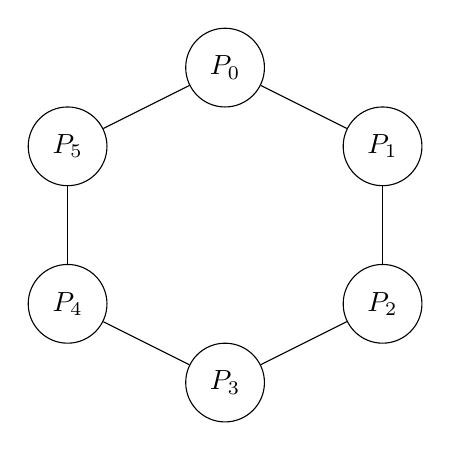
\begin{tikzpicture}
    \node[circle,draw, minimum size=1cm] (0) at (0,2) {$P_0$};
    \node[circle,draw, minimum size=1cm] (1) at (2,1) {$P_1$};
    \node[circle,draw, minimum size=1cm] (2) at (2,-1) {$P_2$};
    \node[circle,draw, minimum size=1cm] (3) at (0, -2) {$P_3$};
    \node[circle,draw, minimum size=1cm] (4) at (-2,-1) {$P_4$};
    \node[circle,draw, minimum size=1cm] (5) at (-2, 1) {$P_5$};
    \draw (0) -- (1); \draw (1) -- (2); \draw (2) -- (3); 
    \draw (3) -- (4); \draw (4) -- (5); \draw (5) -- (0);
\end{tikzpicture}
\vspace*{\fill}
\end{multicols}

\subsection{Conclusiones}

Desde el punto de vista de la cantida de mensajes enviados y la eficiencia, podemos obtener las siguientes conclusiones para las soluciones descriptas.

{\renewcommand{\arraystretch}{2}%\
\begin{center}
\begin{tabular}{p{2.5cm} p{3cm} p{1.8cm} p{7.5cm} }
\textbf{Solución} &  \textbf{\# Mensajes} & \textbf{Orden} & \textbf{Conclusión} \\
\textbf{Centralizada} & $2(n-1)$ & Lineal \newline $O(n)$ & No hay paralelismo, toda la carga del cómputo recae en CentralPeer. Menor overhead en el pasaje de mensajes. Menor eficiencia a mayor $n$. \\
\hline
\textbf{Simétrica} & $n(n-1)$&  Cuadrático \newline $O(n^2)$& Cómputo paralelo pero, mayor overhead en el pasaje de mensjaes.\\
\hline
\textbf{Circular} &  $2(n-1)$& Lineal \newline $O(n)$ & Cómputo paralelo. Mayor eficiencia para $n$ muy grandes.
\end{tabular}
\end{center}}

Nota: Con la primitiva \textbf{\emph{broadcast}}, la cantidad de mensajes se reduce a $n$ para todos los casos. Lo que hace, dicha primitiva es envíar un mensaje (de forma concurrente) a todos los procesos que escuchen el canal utilizado.

\chapter{PMS - Pasaje de Mensajes Asincrónico}

\section{CSP y Comunicación guardada}

Con CSP (\textbf{\emph{Communicating Sequential Processes}}) se introduce el concepto de \textbf{\emph{PMS y comunicación guardada}}. Los procesos, se enviarán mensajes. entre ellos, mediante links directos. La forma general de comunicación, entre procesos, en CSP es de la siguiente forma:

\begin{lstlisting}
DestinationProc!portName(...);
SourceProc?portName(...);
\end{lstlisting}

Siendo los operadores \textbf{\emph{!}} y \textbf{\emph{?}} para el envío y recepción de mensajes respectivamente. Dos procesos, entablabran comunicación cuando ejecuten sentencias de comunicación que hagan match entre sí. 

El siguiente ejemplo, muestra un proceso (Copy) que copia caracteres entre 2 (dos) procesos East y West.

\begin{lstlisting}
Process Copy

Char c;

while (true)
    west?(c)
    east!(c);
end.

End.
\end{lstlisting}

La principal limitación de \textbf{\emph{!}} y \textbf{\emph{?}} es que, son primitivas bloqueantes. Usualmente, se desea, que un proceso pueda comunicarse con los demás; sin importar el orden en que los otros quieran comunicarse con el.

Por ejemplo, si modificamos el ejemplo de Copy de forma tal que; ahora se deben copiar de a 2 caracteres. El proceso Copy, entonces, debe esperar a recibir los 2 caracteres desde West, antes de retransmitirlos. Esto provoca que, East quede bloqueado.

\begin{lstlisting}
Process Copy

Char c1, c2;

while (true)
    west?(c1); west?(c2);
    east!(c1); east!(c1);
end.

End.
\end{lstlisting}

\textbf{\emph{La comunicación guardada}}, ofrece un tipo de \textbf{\emph{comunicación no determinística}} que resuelve la limitación planteada. \textbf{\emph{Combinando sentencias condicionales y de comunicación}} de la siguiente forma $B; C \rightarrow S $, donde:

\begin{itemize}
    \item \textbf{\emph{B}} es una sentencia condicional, que de no existir se asume \emph{verdadera}.
    \item \textbf{\emph{C}} es una sentencia de comunicación.
    \item \textbf{\emph{D}} es un conjunto de sentencias a ejecutar.
    \item Juntas \textbf{\emph{B}} y \textbf{\emph{C}} forman una \textbf{\emph{guarda}} que "protegen" la ejecución de \textbf{\emph{S}}
\end{itemize}

Con respecto al funcionamiento de las \textbf{\emph{guardas}}, se debe tener en cuenta lo siguiente:

\begin{itemize}
    \item La guarda tiene \textbf{\emph{éxito}} si, \textbf{\emph{B}} es verdadera y \textbf{\emph{C}} no causa demora (tiene mensajes $\rightarrow$ ejecución inmediata).
    \item La guarda \textbf{\emph{falla}} si, \textbf{\emph{B}} es falsa.
    \item La guarda se \textbf{\emph{bloquea}} si, \textbf{\emph{B}} es verdadera y \textbf{\emph{C}} causa demora.
\end{itemize}

Podemos aplicar comunicación guardada sobre 2 (dos) tipos de estructuras del control: el \textbf{\emph{if}} y el \textbf{\emph{do}}. Cada una, con la siguiente semántica de ejecución:

\begin{itemize}
    \item Si \textbf{\emph{todas las guardas fallan}} (en simultáneo); la estructura de control finaliza sin efectos.
    \item Si al menos una guarda tiene éxito; se elige una de manera no deterministica, se ejecuta su \textbf{\emph{B}} y luego su \textbf{\emph{C}}. En el caso del \textbf{\emph{if}}, la estructura finaliza.
    \item Si todas las \textbf{\emph{guardas están bloqueadas}}; se espera hasta que alguna tenga éxito.
\end{itemize}

La versión del proceso Copy, para 2 caracteres, se puede mejorar utilizando comunicación guardada del siguiente modo:

\begin{lstlisting}
Process Copy

char c1, c2;
west?(c1);

do  true; west?(c2) -> east!(c1); c1=c2;
[]  true; east!(c1) -> west?(c1);
end;

End.
\end{lstlisting}

Aplicando comunicación guardada, el proceso \emph{Copy}, una vez recibido el primer caracter podrá (de forma no determinística) esperar al segundo caracter o enviar el primero a \emph{East}.
De esta forma, logramos reducir el bloqueo en la comunicación entre \emph{Copy} y \emph{East}.

\chapter{RPC, Rendezvous y Notaciones primitivas}

\section{Introducción}

La técnica de pasaje de mensajes, resulta óptima para resolver problemas del tipo productores/consumidores y pares que interactúan. Ya que, estos plantean un tipo de comunicación unidireccional entre procesos.

No obstante, el uso de esta técnica para problemas del tipo cliente/servidor; no resulta del todo óptima. Ese tipo de problemas supone una comunicación bidireccional. Es decir, un cliente realiza una petición y, posteriormente, un servidor le otorga una respuesta. Esto nos obliga a definir un gran número de canales:

\begin{itemize}
    \item Al menos 1 (un) canal por el cual, el servidor reciba peticiones.
    \item Un canal de respuesta para cada cliente.
\end{itemize}

Los mecanismos de \textbf{\emph{RPC}} y \textbf{\emph{Rendezvous}}, resuelven de forma más adecuada los problemas del tipo cliente/servidor. Combinando PMS con aspectos de monitores.

Como en \textbf{\emph{monitores}}, un módulo (o proceso) expone operaciones públicas. Dichas operaciones, son invocadas por otro módulo (o proceso) utilizando la sentencia \textbf{\emph{call}}.

Como en \textbf{\emph{PMS}}, la eejcución de una sentencia \textbf{\emph{call}} demora al llamador hasta obtener una respuesta.

Las \textbf{\emph{operaciones}}, resultan \textbf{\emph{canales de comunicación bidireccional}}. Desde el llamador hacia el proceso que sirve la llamada, y luego, de vuelta al llamador.


\section{Remote Procedure Calls (RPC)}

Los programas se descomponen en módulos (con procesos y procedimientos). Los procesos, de un módulo, son llamados \textbf{\emph{background}} para diferenciarlos de los procesos exportados (\textbf{\emph{servers}}). El siguiente ejemplo, muestra de forma trivial la especificación de un módulo.

\begin{lstlisting}
Module module_name
    op opname(params)[returns type];        # (1) Interfaz publica
Body
    int x;                                  # (2) Definicion de variables locales
    x = 0;                                  # e inicializacion    

    proc opname(params)[returns type]       # (3) Definicion de procedimientos exportados
    begin
        # Cuerpo del procedimiento.
    end;

    proc local_proc(params)[returns type]   # (4) Definicion de procedimientos locales
    begin
        # Cuerpo del procedimiento.
    end;

    Process Main                            # (5) Definicion de procesos locales
        # Cuerpo del proceso bakground
    end;
End module_name;
\end{lstlisting}

Los procesos background tienen acceso a las variables y pueden invocar procedimientos del mismo módulo. A su vez, como sucede en monitores, pueden invocar procedimientos definidos en otros módulos. Siempre y cuando, estos últimos, sean exportados por dicho módulo.

La ejecución de una llama intermódulo, difiere con respecto a una local.

\begin{itemize}
    \item Un nuevo proceso atiende la llamada y los argumentos son pasados como mensajes entre el llamador y el proceso servidor.
    \item El proceso llamador que demorado mientras se ejecuta el cuerpo del procedimiento invocado.
    \item Cuando el proceso servidor finaliza su ejecución del procedimiento invocado, retorna los resultados y finaliza.
    \item El proceso llamador, continua su ejecución.
\end{itemize}

\centerline{
    \includegraphics[width=4in, height=1.5in]{assets/rpc_execution.png}
}

\subsection{Sincronización}

Con RPC, la \textbf{\emph{sincronización entre proceso llamador y servidor está implícita}}. No obstante, necesitamos mecanismos para que procesos server y background sincronicen dentro de un módulo. Existen 2 (dos) enfoques para proveer sincronización dentro de un módulo.


\begin{multicols}{2}
\centerline{\textbf{\emph{A lo sumo, un proceso activo}}}

\centering
Apropidado para entornos monoprocesador ya que, reduce el context switch.

\begin{itemize}
    \item Mutex $\rightarrow$ Implícito.
    \item Condición $\rightarrow$ Explícito (semáforos o monitores).
\end{itemize}

\columnbreak
\centerline{\textbf{\emph{Ejecución concurrente}}}

Apropidado, de forma natural, para entornos multriprocesador.

\begin{itemize}
    \item Mutex $\rightarrow$ Explícito (semáforos o monitores).
    \item Condición $\rightarrow$ Explícito (semáforos o monitores).
\end{itemize}

\end{multicols}

\subsection{Time Server}

El siguiente módulo es una adaptación del ejemplo del libro.

\begin{lstlisting}
module TimeServer

op get_time(): int;
op delay(int interval);

body

int time = 0;                   # Tiempo inicial del TimeServer (en ms).
Queue delayed(waketime, id);    # Cola de procesos dormidos, por la operacion delay.
Sem m = 1;                      # Semaforo para garantizar mutex, en el acceso a delayed.
Sem d = ([n] 0);                # Arreglo de semaforos para demorar procesos.

proc get_time(): int            # Retorna el tiempo actual del servidor en ms.
    return time;
end;

proc delay(int interval)        # Demora un proceso tantos ms, como interval lo indique.
    P(m);
    waketime = time + interval;
    delayed.push(waketime, id);
    V(m);
    P(d[id]);
end;

process Clock                   # Proceso background. Mantiene actualizada la variable time
    while (true)                # y despierta procesos demorados por la operacion delay.
        time++;                 
        P(m);
        while (time >= menor waketime en delayed)
            delayed.pop(waketime, id);
            V(d[id]);
        end;
        V(m);
    end;
end;
End.
\end{lstlisting}

\section{Rendezvous}

Al igual que RPC, el programa se descompone en módulos, se brindan los mecanismos para la \textbf{\emph{comunicación intermódulo}} y se demoran a los procesos llamadores.

La cabecera de un módulo, debe especificar las operaciones exportadas. Mientras que el cuerpo, del módulo, contendrá \textbf{\emph{un único proceso}}; que atenderá las llamadas a las operaciones en lugar de crear un nuevo proceso servidor.

Dicho proceso, esperara por una call y actuar. Las llamadas, a operaciones, serán atendidas de a una por vez aunque los procesos se ejecuten concurrentemente. Esto \textbf{\emph{provee sincronización dentro del módulo}}.

\centerline{
    \includegraphics[width=4in, height=1.5in]{assets/rendezvous_execution.png}
}

\subsection{Sentencias Input}

Suponiendo que, un módulo exporta la siguiente operación: \lstinline{op opname(formals)}. El proceso servidor realiza rendezvous con un llamador de \lstinline{opname}, ejecutando una sentencia \textbf{\emph{input}}. Dicha sentencia, respeta la siguiente forma:

\begin{lstlisting}
in opname(formals) -> S; ni
\end{lstlisting}

Las partes entre \lstinline{in} y \lstinline{ni} son conocidas como \textbf{\emph{operaciones guardadas}}. La guarda nombra las operaciones y provee sus parámetros.
En cuanto a \lstinline{S}, es un conjunto de sentencias a ejecutar en la invocación de la operación. Los parámetros, de la operación, tienen alcance de a toda la guarda; por consiguente \lstinline{S} podrá leer y escribir sus valores.

Una sentencia \lstinline{input}, demora al proceso servidor hasta que haya al menos una llamada pendiente a \lstinline{opname}. Entonces, elige la llamada pendiente más antigua, copia los argumentos en los parámetros formales, ejecuta \lstinline{S} y finalmente, retorna los resultados al proceso llamador.

Es posible ofrecer \textbf{\emph{comunicación guardada}}, en una sentencia \lstinline{input} de la siguiente forma:


\begin{lstlisting}[escapeinside={(*}{*)}]
In opname(*$_1$*) (formals) and B(*$_1$*) by E(*$_1$*) -> S(*$_1$*)
[] opname(*$_2$*) (formals) and B(*$_2$*) by E(*$_2$*) -> S(*$_2$*)
Ni
\end{lstlisting}

Donde \textbf{\emph{E}} supone una \textbf{\emph{condicion booleana de sincronización}}. Mientras que, \textbf{\emph{E}} una \textbf{\emph{expresión de scheduling}}. Ambas expresiones son opcionales.

\subsection{Buffer limitado}

\begin{lstlisting}
Module Buffer

op depositar(int);
op retirar(int);

Body
Process Buffer
    Queue buffer;
    int cant = 0;
    int cantMax = n;

    while(true)
        in depositar(x) and (cant < cantMax) ->
            buffer.push(x);
            cant++;
        [] retirar(x) and (cat > 0) ->
            buffer.pop(x);
            cant--
        ni
    end;
end;
End.
\end{lstlisting}

\subsection{ADA}

Un programa, escrito en ADA, está compuesto por subprogramas, paquetes y tareas. Donde \textbf{\emph{rendezvous}} es el principal mecanismo de comunicación y sincronización.

Las tareas (\textbf{\emph{tasks}}), son procesos independientes que cuentan con una especificación y un cuerpo (\textbf{\emph{body}}). En la especificación, se definen las operaciones visibles por otros procesos (\textbf{\emph{entry}}). El cuerpo, contiene variables locales (junto con su inicialización) y sentencias de atención (\textbf{\emph{entry calls}}).

\begin{lstlisting}
Procedure nombreProceso

Task nombreTarea Is
    # Declaracion de entries
end;

Task Body nombreTarea Is
    # Declaracion de locales e inicializacion
Begin
    # Sentencias ...
end;

End nombreProceso;
\end{lstlisting}

Un programa en ADA, atiende solicitudes a procedimientos mediante la sentencia \lstinline{accept}. La cual equivale a \lstinline{input} pero, su ejecución es determinística y no posee guardas. Dicha sentencia, posee la siguiente forma:

\begin{lstlisting}
Accept E (formals) do
    # Sentencias
end;
\end{lstlisting}

De ser necesario, comunicación guardada con un comportamiento no determinístico. ADA ofrece la sentencia \lstinline{select}. No obstante, \lstinline{select} resulta menos poderosa que la notación formal establecida en rendezvous; por 2 (dos) motivos.

\begin{enumerate}
    \item No soporta expresiones de scheduling.
    \item La expresión de sincronización, no puede referenciar a los parámetros formales de la operación.
\end{enumerate}

\subsection{Buffer limitado con ADA}

\begin{lstlisting}
Procedure nombreProceso

Task Mailbox Is
    Entry Depositar (msg: IN string)
    Entry Retirar (msg: OUT string)
End;
    
Task Body Mailbox Is
    Array datos[n];
    Int count, first, last = 0;
Begin
    Loop
        Select
            When (count < n) -> Accept Depositar (msg: IN string)
                # Sentencias de la operacion Depositar
            End Depositar;
            Or
            When (count > 0) -> Accept Retirar (msg: OUT string)
                # Sentencias de la operacion Retirar
            End Retirar;
        End;
    End;
End;
End nombreProceso;
\end{lstlisting}

\section{Notaciones primitivas}

Mecanismo que \textbf{\emph{combina RPC, Rendezvous y PMA en un paquete coherente}}. Con este mecanismo, será posible implementar una solución óptima al problema de filtros y pares que interactúan mediante el uso de las técnicas de RPC y Rendezvous.

Los programas, son colecciones de módulos que exportan operaciones visibles para otros módulos o procesos.

Una operación puede ser invocada por call (sincrónico) o por send (asincrónico). Como también una operación puede ser servida por RPC o Rendezvous (según la elección del programador del módulo).

{\renewcommand{\arraystretch}{2}%\
\begin{center}
    \begin{tabular}{c c c}
    \textbf{Invocación} &  \textbf{Servicio} & \textbf{Efecto} \\
    call & proc & Llamado a procedimiento. \\
    \hline
    call & in & Rendezvous. \\
    \hline
    send & proc & Creación dinámica de un proceso. \\
    \hline
    send & in & PMA. \\
\end{tabular}
\end{center}}

\chapter{Paradigmas de intercacción entre procesos}

\section{Introducción}

Existen 3 (tres) esquemas básicos de interacción entre procesos: productores/consumidores, cliente/servidor y pares que interactúan. Estos esquemas básicos se pueden combinar de muchas maneras, dando lugar a nuevos modelos o paradigmas de interacción entre procesos.

\section{Manager and workers}

Es la implementación distribuida del modelo \textbf{\emph{bag of tasks}}. Diversos procesos workers comparten una bolsa de tareas. Cada worker repetidamente toma una tarea de la bolsa, la ejecuta y posiblemente genere una (o más) tareas nuevas para depositar en la bolsa.

La principal ventaja de este paradigma, en cuanto a cómputo paralelo, es la facilidad para escalar y balancear la carga de trabajo de cada worker.

Por el otro lado un proceso manager representa la bolsa de tareas. Es decir, mantiene la lista de tareas, recolecta los resultados y detecta la finalización de todas las tareas.

En escencia, un manager funciona como un server. Mientras que, un worker como un cliente.

\textbf{Caso de uso}: multiplicación de matrices.

\section{Heartbeat}

Los procesos, periódicamente, deben intercambiar información con mecanismos de tipo send/receive.

En particular, puede ser utilizado cuando los datos están divididos entre los procesos workers. Donde, cada worker es responsable de actualizar una parte de los datos. Dicha actualización, dependerá de los valores que contenga cada worker o sus vecinos inmediatos.

La lógica de este paradigma, tiene relación con su nombre. Los procesos se expanden enviando información a sus vecinos y se contraen recibiendo información actualizada desde sus vecinos.

La interacción entre vecinos, dada por la disposición de las primitivas send/receive, produce una especie de barrera de sincronización entre ellos. Impidiendo que, cada worker inicie su fase de actualización antes de que su vecino no finalice la suya.

\textbf{Caso de uso}: paralelizar soluciones iterativas $\rightarrow$ topología de una red, procesamiento de imágenes.

\section{Pipeline}

Los procesos, funcionan como filtros y se encuentran conectados entre sí; formando una colección de filtros. De esta manera, la información fluye por los procesos utilizando alguna forma de receive/send. Existen 3 (tres) formas de conectar los procesos:

\begin{multicols}{2}

\textbf{Pipeline Abierto}

La fuente de entrada y salida, del pipeline, no está especificada.

\columnbreak
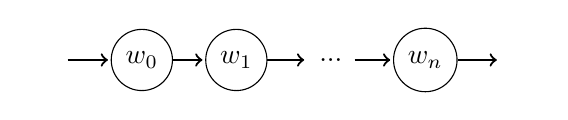
\begin{tikzpicture}
    \node[circle,draw=none, minimum size=0.5cm] (in) at (0,0) {};
    \node[circle,draw, minimum size=0.5cm] (worker0) at (1.2,0) {$w_0$};
    \node[circle,draw, minimum size=0.5cm] (worker1) at (2.4,0) {$w_1$};
    \node[circle,draw=none, minimum size=0.5cm] (workerX) at (3.6,0) {...};
    \node[circle,draw, minimum size=0.5cm] (workerN) at (4.8,0) {$w_n$};
    \node[circle,draw=none, minimum size=0.5cm] (out) at (6,0) {};
    \draw[thick] (in) edge[post] (worker0);
    \draw[thick] (worker0) edge[post] (worker1);
    \draw[thick] (worker1) edge[post] (workerX);
    \draw[thick] (workerX) edge[post] (workerN);
    \draw[thick] (workerN) edge[post] (out);
\end{tikzpicture}
\end{multicols}

\begin{multicols}{2}

\textbf{Pipeline Cerrado}

Pipeline abierto conectado por un coordinador. El coordinador, produce los datos de entrada para $w_0$ y consume la salida de $w_n$.

\columnbreak
\begin{tikzpicture}
    \node[circle,draw=none, minimum size=0.5cm] (in) at (0,0) {};
    \node[circle,draw, minimum size=0.5cm] (worker0) at (1.2,0) {$w_0$};
    \node[circle,draw, minimum size=0.5cm] (worker1) at (2.4,0) {$w_1$};
    \node[circle,draw=none, minimum size=0.5cm] (workerX) at (3.6,0) {...};
    \node[circle,draw, minimum size=0.5cm] (workerN) at (4.8,0) {$w_n$};
    \node[ellipse,draw, minimum size=1cm] (coordinator) at (3,-1.2) {$cordinator$};

    \draw[thick] (coordinator) edge[post, bend left=30] (worker0);
    \draw[thick] (worker0) edge[post] (worker1);
    \draw[thick] (worker1) edge[post] (workerX);
    \draw[thick] (workerX) edge[post] (workerN);
    \draw[thick] (workerN) edge[post, bend left=30] (coordinator);
\end{tikzpicture}
\end{multicols}

\begin{multicols}{2}

    \textbf{Pipeline Circular}
    
    La salida de $w_n$ está conectada a la entrada de $w_0$. Útil cuando la solución, no puede obtenerse en una sola pasada.
    
    \columnbreak
    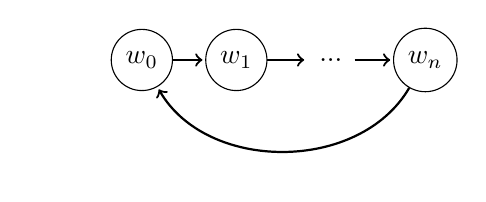
\begin{tikzpicture}
        \node[circle,draw=none, minimum size=0.5cm] (in) at (0,0) {};
        \node[circle,draw, minimum size=0.5cm] (worker0) at (1.2,0) {$w_0$};
        \node[circle,draw, minimum size=0.5cm] (worker1) at (2.4,0) {$w_1$};
        \node[circle,draw=none, minimum size=0.5cm] (workerX) at (3.6,0) {...};
        \node[circle,draw, minimum size=0.5cm] (workerN) at (4.8,0) {$w_n$};
    
        \draw[thick] (worker0) edge[post] (worker1);
        \draw[thick] (worker1) edge[post] (workerX);
        \draw[thick] (workerX) edge[post] (workerN);
        \draw[thick] (workerN) edge[post, bend left=60] (worker0);
    \end{tikzpicture}
\end{multicols}

\section{Probes and echoes}

La interacción entre procesos permite recorrer estructuras dinámicas, diseminando y recolectando información.

La estructura de muchos programas distribuidos, puede verse como árboles o gráfos. En el cual, los procesos son nodos y los canales aristas.

Una primitiva \textbf{\emph{probe}} es un mensaje enviado por un nodo, a todos sus sucesores. Mientras que, una primitiva \textbf{\emph{echo}} es su respectiva respuesta. Este paradigma, es el análogo al algoritmo Deep Search First (DFS).

\textbf{Caso de uso}: Cuando se desea recorrer una red, de la cual no se conoce la cantidad de nodos $\rightarrow$ redes móviles.

\section{Broadcasts}

Los procesos suelen enviar mensajes a todos los demás, de forma paralela, mediante una primitiva \textbf{\emph{broadcast}}. 

Dicha primitiva, no se asume atómica, por lo cual los procesos pueden recibir los mensajes en distinto orden al cual fueron enviados. La primitiva \textbf{\emph{receive}} funciona de manera tradicional, sobre el canal de cada proceso.

\textbf{Caso de uso}: Mensaje broadcast en redes LAN.

\section{Token passing}

Lo procesos se pasan, entre sí, un token que garantiza el acceso exclusivo a un recurso compartido.

\textbf{Caso de uso}: Exclusión mutua en ambientes distribuidos $\rightarrow$ Exclusión mutua con toke ring.

\subsection{Exclusión mutua con toke ring}

Existe un proceso \emph{helper} por cada proceso que quiera solicitar acceso a una SC. Los procesos \emph{helper}, esperan por una solicitud de acceso (\emph{entryRequest}).

En caso de tener solicitudes pendientes (y poseer el token), concederán el acceso al proceso correspondiente (\emph{grant}). Luego, esperaran a recibir una solicitud de salida (\emph{exitRequest}).

Una vez finalizada la atención, pasarán el token al proceso \emph{helper} siguiente.

\begin{lstlisting}[multicols=2]
# Exclusion mutua con toke ring (PMA).
Chan token[n];
Chan entryRequest[n];
Chan exitRequest[n];
Chan grant[n];

Process Worker[i=1..n]
while(true)
    send entryRequest[i]();
    receive grant[i]();
    # Seccion Critica ...
    send exitRequest[i];
end;
end;

Process Helper[i=1..n]
while(true)
    receive token[i]();
    if (!empty(entryRequest[i]))
        receive entryRequest[i]();
        send grant[i]();
        receive exitRequest[i]();
    end;
    send token[(i mod n) + 1]();
end;
end;
\end{lstlisting}

\section{Servidores replicados}

Los procesos servidores gestionan el acceso a un recurso. Al existir $n$ instancias del recurso, se replicará un servidor por cada una. También, puede utilizarse para abstraer a los clientes la cantidad real de recursos.

\textbf{Caso de uso}: En el problema de los filósofos, estos le solicitan sus cubiertos (recursos) a un mozo (servidor). Los filósofos, desconocen la existencia de cubiertos ajenos.

\end{document}